%%
%% Automatically generated file from DocOnce source
%% (https://github.com/hplgit/doconce/)
%%
%%
% #ifdef PTEX2TEX_EXPLANATION
%%
%% The file follows the ptex2tex extended LaTeX format, see
%% ptex2tex: http://code.google.com/p/ptex2tex/
%%
%% Run
%%      ptex2tex myfile
%% or
%%      doconce ptex2tex myfile
%%
%% to turn myfile.p.tex into an ordinary LaTeX file myfile.tex.
%% (The ptex2tex program: http://code.google.com/p/ptex2tex)
%% Many preprocess options can be added to ptex2tex or doconce ptex2tex
%%
%%      ptex2tex -DMINTED myfile
%%      doconce ptex2tex myfile envir=minted
%%
%% ptex2tex will typeset code environments according to a global or local
%% .ptex2tex.cfg configure file. doconce ptex2tex will typeset code
%% according to options on the command line (just type doconce ptex2tex to
%% see examples). If doconce ptex2tex has envir=minted, it enables the
%% minted style without needing -DMINTED.
% #endif

% #define PREAMBLE

% #ifdef PREAMBLE
%-------------------- begin preamble ----------------------

\documentclass[%
oneside,                 % oneside: electronic viewing, twoside: printing
final,                   % draft: marks overfull hboxes, figures with paths
10pt]{article}

\listfiles               %  print all files needed to compile this document

\usepackage{relsize,makeidx,color,setspace,amsmath,amsfonts,amssymb}
\usepackage[table]{xcolor}
\usepackage{bm,ltablex,microtype}

\usepackage[pdftex]{graphicx}

\usepackage[T1]{fontenc}
%\usepackage[latin1]{inputenc}
\usepackage{ucs}
\usepackage[utf8x]{inputenc}

\usepackage{lmodern}         % Latin Modern fonts derived from Computer Modern

% Hyperlinks in PDF:
\definecolor{linkcolor}{rgb}{0,0,0.4}
\usepackage{hyperref}
\hypersetup{
    breaklinks=true,
    colorlinks=true,
    linkcolor=linkcolor,
    urlcolor=linkcolor,
    citecolor=black,
    filecolor=black,
    %filecolor=blue,
    pdfmenubar=true,
    pdftoolbar=true,
    bookmarksdepth=3   % Uncomment (and tweak) for PDF bookmarks with more levels than the TOC
    }
%\hyperbaseurl{}   % hyperlinks are relative to this root

\setcounter{tocdepth}{2}  % levels in table of contents

% Tricks for having figures close to where they are defined:
% 1. define less restrictive rules for where to put figures
\setcounter{topnumber}{2}
\setcounter{bottomnumber}{2}
\setcounter{totalnumber}{4}
\renewcommand{\topfraction}{0.95}
\renewcommand{\bottomfraction}{0.95}
\renewcommand{\textfraction}{0}
\renewcommand{\floatpagefraction}{0.75}
% floatpagefraction must always be less than topfraction!
% 2. ensure all figures are flushed before next section
\usepackage[section]{placeins}
% 3. enable begin{figure}[H] (often leads to ugly pagebreaks)
%\usepackage{float}\restylefloat{figure}

% prevent orhpans and widows
\clubpenalty = 10000
\widowpenalty = 10000

\newenvironment{doconceexercise}{}{}
\newcounter{doconceexercisecounter}


% ------ header in subexercises ------
%\newcommand{\subex}[1]{\paragraph{#1}}
%\newcommand{\subex}[1]{\par\vspace{1.7mm}\noindent{\bf #1}\ \ }
\makeatletter
% 1.5ex is the spacing above the header, 0.5em the spacing after subex title
\newcommand\subex{\@startsection{paragraph}{4}{\z@}%
                  {1.5ex\@plus1ex \@minus.2ex}%
                  {-0.5em}%
                  {\normalfont\normalsize\bfseries}}
\makeatother


% --- end of standard preamble for documents ---


% insert custom LaTeX commands...

\raggedbottom
\makeindex
\usepackage[totoc]{idxlayout}   % for index in the toc
\usepackage[nottoc]{tocbibind}  % for references/bibliography in the toc

%-------------------- end preamble ----------------------

\begin{document}

% matching end for #ifdef PREAMBLE
% #endif

\newcommand{\exercisesection}[1]{\subsection*{#1}}


% ------------------- main content ----------------------



% --- begin exercise ---
\begin{doconceexercise}
\refstepcounter{doconceexercisecounter}

\exercisesection{Exercise \thedoconceexercisecounter: Modelling a 3D ion trap}


\emph{(Made by René Ask)}


In 1989, Wolfgang Paul and Hans Georg Dehmelt received a Nobel prize in physics for the creation of the \emph{Paul trap} (although the actual trapping technique was developed by them back in the 1950s). The trapping technique allows physicists to trap and study properties of particles and atoms predicted by quantum mechanics.
For instance, at CERN physicists trap antiparticles using such a trap to measure their properties and compare them with theoretical predictions. Such traps can also be used to trap the fundamental computing units in quantum computers, known as \emph{qubits}.

In this exercise, we'll look at how we can go about and create such a trap with theory from electromagnetism. For our purpose we'll assume we're going to trap ions with a charge $q > 0$ and mass $m$. We'll assume that the trap is in a vacuum with no charge distibution within.


\subex{a)}
Imagine we want the particle to stay located in a small area in space. The simplest such area to represent mathematically would be a sphere, wouldn't it? To create a spherical trap, we can imagine that we set up a continuous distribution of charges to create a spherical harmonic oscillator (kinda like three decoupled springs with a mass attached to each) such that its potential is
\begin{equation}
  V(x,y,z) = A(x^2 + y^2 + z^2),
\end{equation}
for an appropriate constant $A$. This way the particle would oscillate back and forth about the origin with certainty. Unfortunately, nature is not that simple. Show that this potential cannot exist in a vacuum.

% --- begin hint in exercise ---

\paragraph{Hint.}
Use Laplace's equation.

% --- end hint in exercise ---


% --- begin solution of exercise ---
\paragraph{Solution.}
Laplace's equation is given by $\nabla^2 V = 0$ (recall that we assume there's no free charges inside the trap, so $\rho = 0$).
\begin{equation}
  \nabla^2 V = \frac{\partial^2 V}{\partial x^2} + \frac{\partial^2 V}{\partial y^2} + \frac{\partial^2 V}{\partial z^2} = 6A \neq 0.
\end{equation}
Since $V$ does not obey Laplace's equation, it's an unphysical electric potential and cannot exist in a vacuum.

% --- end solution of exercise ---

\subex{b)}
To create a potential that can exist in a vacuum, we can modify the former as
\begin{equation}
  V(x,y,z) = A(\alpha x^2 + \beta y^2 + \gamma z^2),
\end{equation}
where $\alpha, \beta, \gamma \neq 0$ are real constants. Find constraints on these constants such that the potential can exist in a vacuum and show that from a suitable choice of constraints we can obtain the potential (there's more than one choice)
\begin{equation}
  V(x,y,z) = A( x^2 +  y^2 - 2z^2),
\end{equation}

% --- begin hint in exercise ---

\paragraph{Hint.}
Again, use Laplace's equation.

% --- end hint in exercise ---


% --- begin solution of exercise ---
\paragraph{Solution.}
The potential must obey Laplace's equation, so
\begin{equation}
  \nabla^2 V =2A(\alpha  + \beta  + \gamma ) = 0,
\end{equation}
which can be achieved if $\beta = \alpha$ and $\gamma = -2\alpha$ (there are several other valid constraints, but these will be more convenient with respect to the geometrical setup of the trap). Setting $\alpha = 1$, we get
\begin{equation}
  V(x,y,z) = A(x^2 + y^2 - 2z^2).
\end{equation}

% --- end solution of exercise ---

\subex{c)}

\begin{figure}[!ht]  % fig:penningtrap_noB
  \centerline{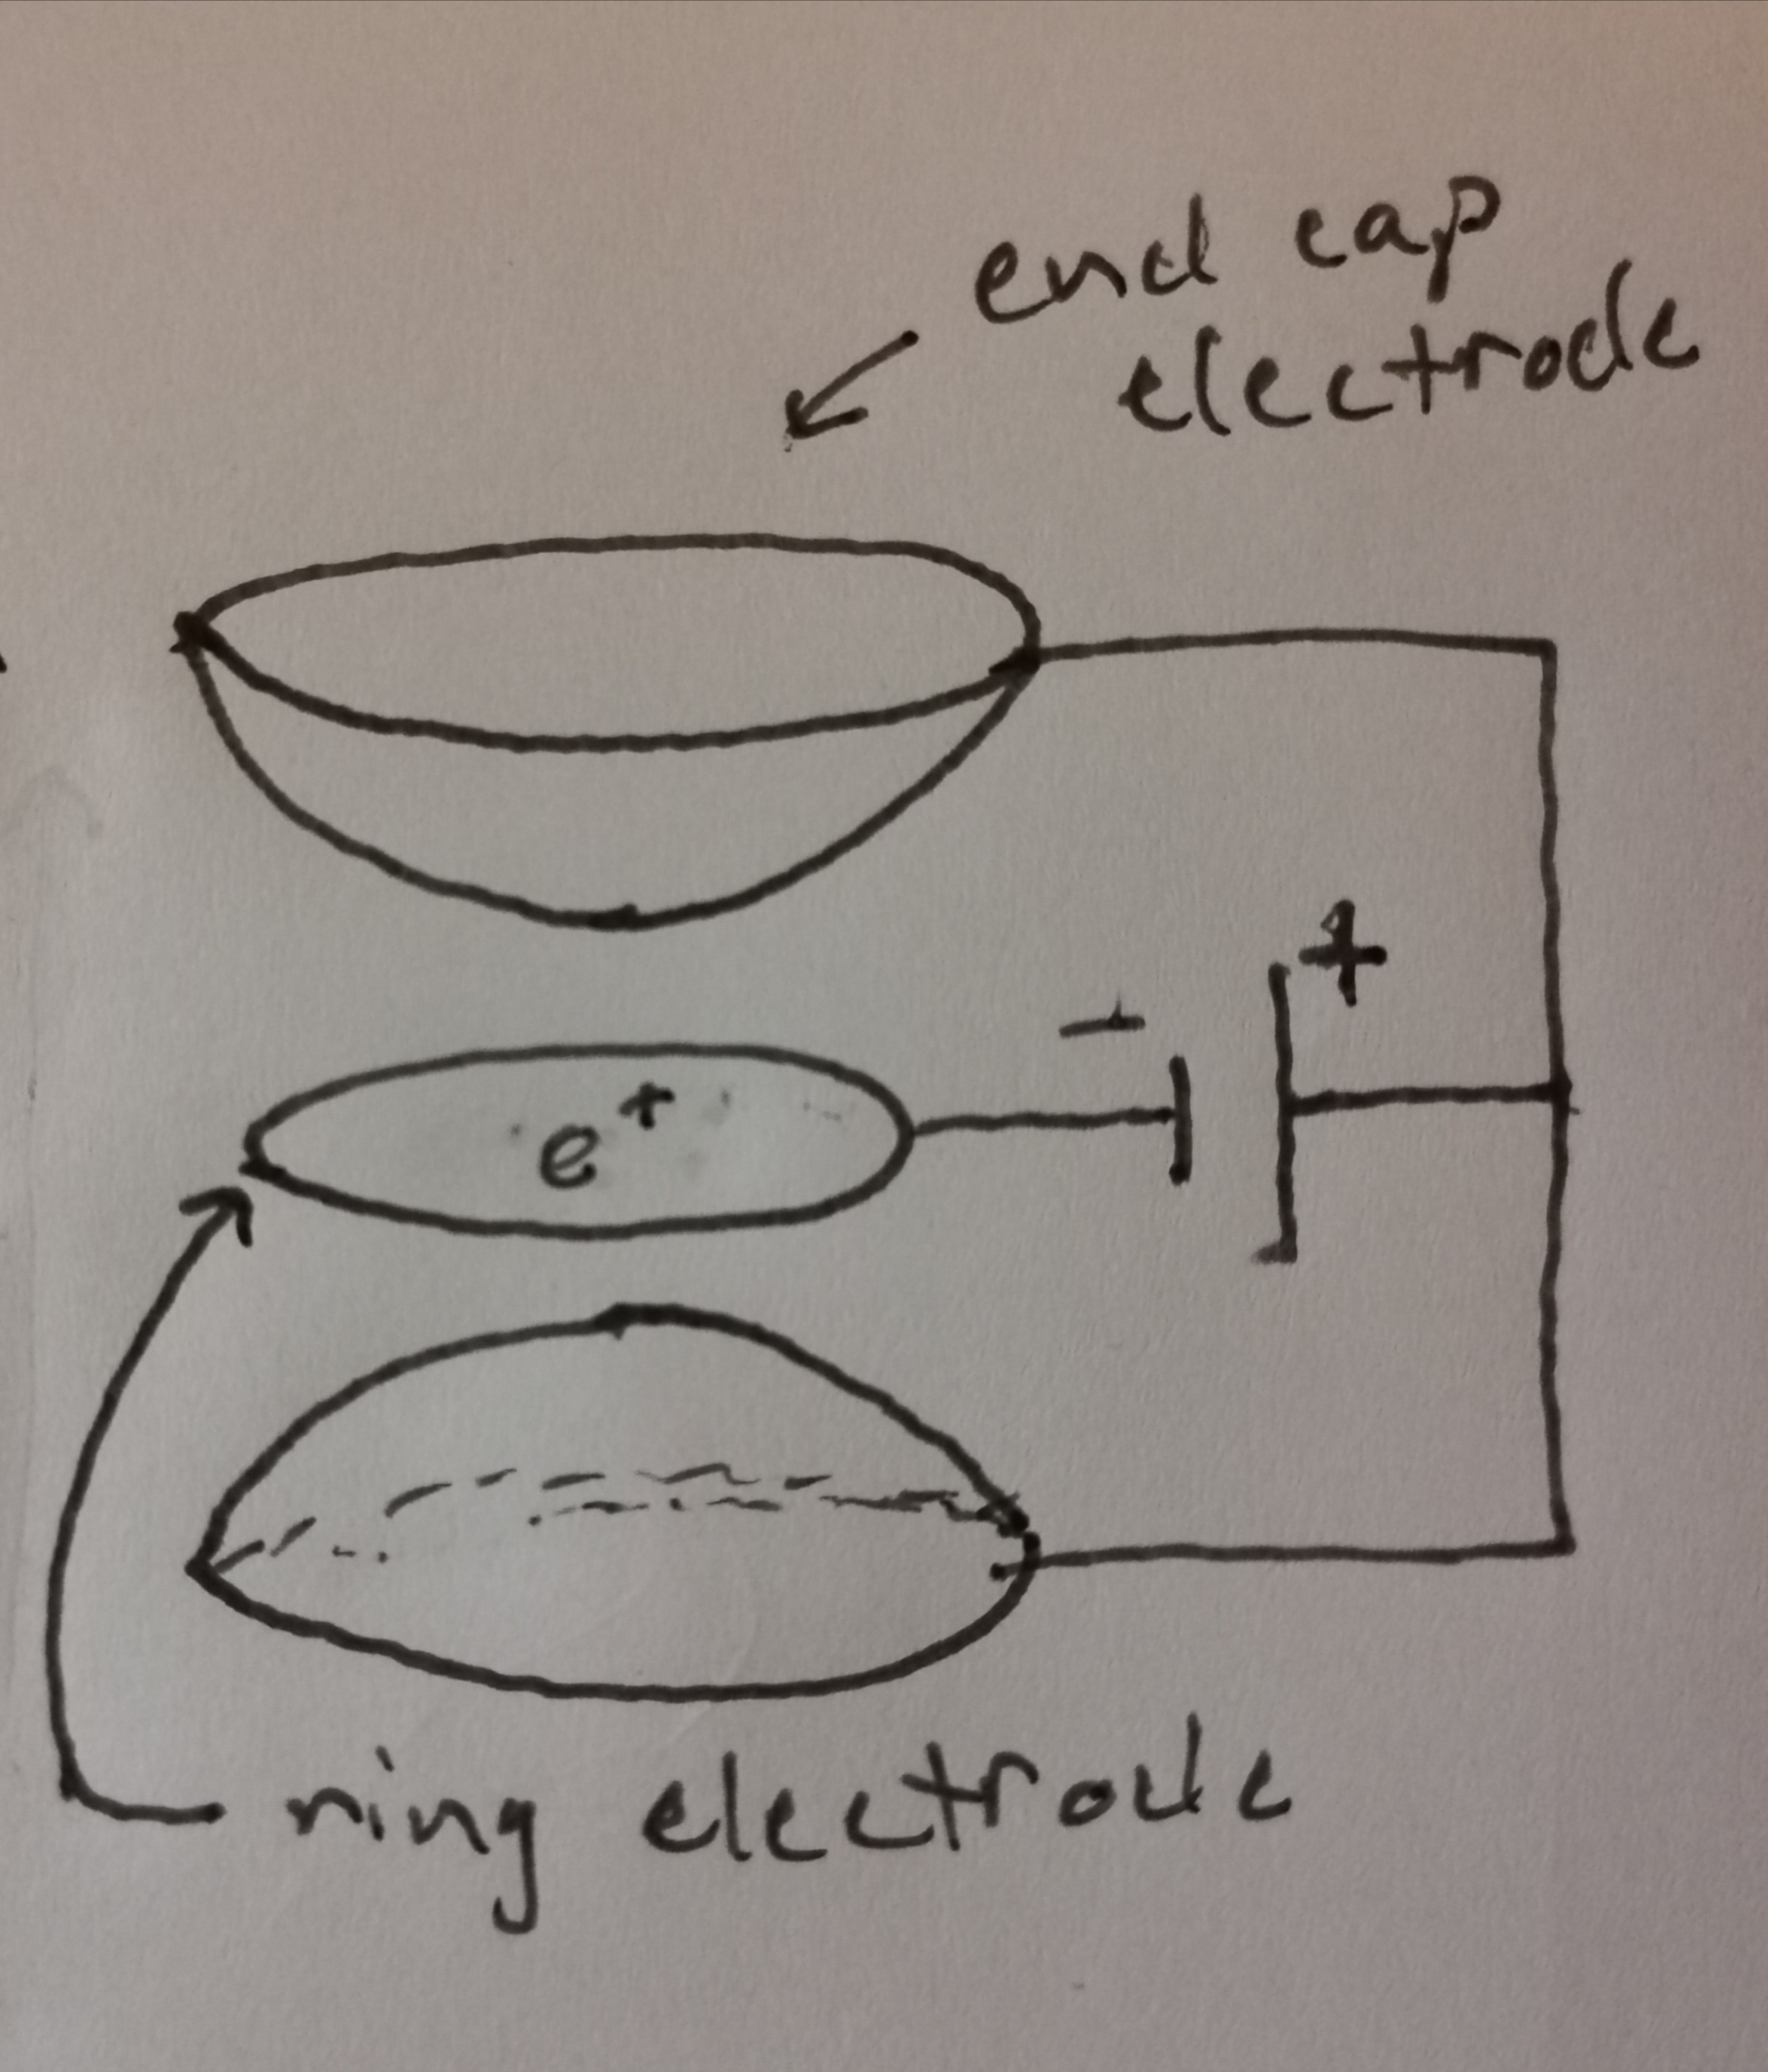
\includegraphics[width=0.5\linewidth]{figures/penningtrap_noB.jpg}}
  \caption{
  A simple setup for the trap with (approximately) the potential $V(x,y,z)$. In reality the end caps must be paraboloids stretching out to infinity. Similarly, the ring must be a hyperboloid that stretches out to infinity in both directions. But inside the setup shown, $V(x,y,z)$ is a good approximation. \label{fig:penningtrap_noB}
  }
\end{figure}
%\clearpage % flush figures fig:penningtrap_noB


Figure~\ref{fig:penningtrap_noB} shows as simple experimental setup consisting of two finite paraboloid-shaped end-caps and a ring which will serve as electrodes. To trap positive ions, we want the end caps to be held at a static positive potential $V_0$ and the ring  to be held at at static negativ potential $-V_0$. Let the radius of the ring be $r_0$ and the end caps be placed a length $z_0$ from the center of the ring. Using cylindrical coordinates $x = r\cos\phi$, $y = r\sin\phi$ and $z = z$, the potential can be written as
\begin{equation}
  V(r,z) = A(r^2 - 2z^2).
\end{equation}
Find the constant $A$ and the relationship between $r_0$ and $z_0$ and use the results to show that the potential for the trap can be written as
\begin{equation}
  V(r,z) = \frac{V_0}{r_0^2}(2z^2 - r^2).
\end{equation}
\emph{(This expression for $V(r,z)$ will to a good degree approximate the actual potential inside the trap.)}


% --- begin solution of exercise ---
\paragraph{Solution.}
The ring is held at a negative potential $-V_0$, so $V(r_0, 0) = -V_0$ which implies
$$ V(r_0, 0) = Ar_0^2 = -V_0 \implies A = -\frac{V_0}{r_0^2}$$
The end caps is held at a positive potential $V_0$, so $V(0,z_0) = V_0$, giving
$$ V(0, z_0) = \frac{V_0}{r_0^2}(2z_0^2) = V_0,$$
meaning $r_0^2 = 2z_0^2$. Clearly, then, the potential can be written as
$$ V(r,z) = \frac{V_0}{r_0^2}(2z^2 - r^2).$$

% --- end solution of exercise ---

\subex{d)}
Show that this potential cannot trap the ion (Ah... that's a bummer, but worry not - we will fix this later on).

% --- begin hint in exercise ---

\paragraph{Hint.}
Use the second derivative test (Hessian determinant). Or plot (google surface plot) it and use it to explain why you can't trap the ion.

% --- end hint in exercise ---


% --- begin solution of exercise ---
\paragraph{Solution.}
The Hessian matrix is given by
$$
H =
  \begin{bmatrix}
    \frac{\partial^2 V}{\partial r^2} & \frac{\partial^2 V}{\partial r \partial z} \\
    \frac{\partial^2 V}{\partial r \partial z} & \frac{\partial^2 V}{\partial z^2}
  \end{bmatrix}
  =
  \begin{bmatrix}
    -\frac{2V_0}{r_0^2} & 0 \\
    0 & \frac{4V_0}{r_0^2}
  \end{bmatrix}
$$
which has the determinant $\det H = -8V_0^2/r_0^4 < 0 $. Since $\det H < 0$, there exists no stable equilibrium for the potential and thus we can't possibly trap the ion.

Plotting the potential $V(r,z)$ would give us figure~\ref{fig:potential}. The code below was used to produce the plot. In the figure, we can see that there's no stable equilibrium points since there
are no local minima. But then we can't hope to successfully trap the particle since there's no point in space the particle will oscillate about.
\begin{verbatim}
  from mpl_toolkits.mplot3d import Axes3D
  import matplotlib.pyplot as plt
  import numpy as np
  fig = plt.figure()
  ax = fig.gca(projection="3d")
  z0 = 1
  r0 = np.sqrt(2)*z0
  r = np.linspace(0, r0,1001)
  z = np.linspace(-z0, z0, 1001)
  r,z = np.meshgrid(r,z)
  V = 2*z*z - r*r
  surf = ax.plot_surface(r,z,V)
  plt.show()
\end{verbatim}


\begin{figure}[!ht]  % fig:potential
  \centerline{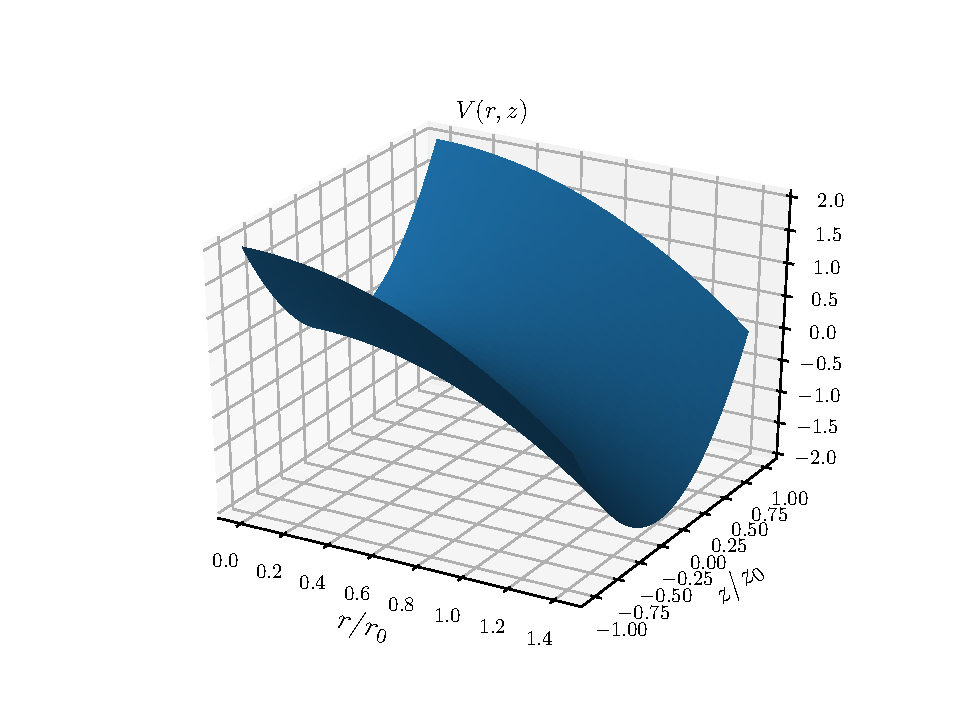
\includegraphics[width=0.8\linewidth]{figures/fig-failed_trap.pdf}}
  \caption{
  The particle would escape since there's no stable equilibrium here. \label{fig:potential}
  }
\end{figure}
%\clearpage % flush figures fig:potential


% --- end solution of exercise ---

\subex{e)}
We may summarize our findings so far: a static electric field is \emph{not} sufficient to trap charged particles in 3D. This is stated by \emph{Earnshaw's theorem}. There's a clever way to fix this problem. Instead of working with a static potential, we replace the constant $V_0$ with the sinusoidal factor $V_0 \cos (\Omega t)$. This way, if we provide an appropriate angular frequency $\Omega$, we can stop the particle(s) in the trap from escaping in the $xy$-plane. The general expression is
\begin{equation}
  V(x,y,z,t) = \frac{V_0\cos \Omega t}{r_0^2}(2z^2 - x^2 - y^2),
\end{equation}
Find the force on a particle with charge $q > 0$ and mass $m$. Solve the equations of motion numerically and plot the particle's trajectory in 3D. Are you able to trap the particle?

% --- begin hint in exercise ---

\paragraph{Hint.}
Use Newton's almighty 2.law! Also, let me suggest some constants for you: Set  $V_0 = 4000$ V, $\Omega = 100\pi$ Hz (that's the angular frequency a wall outlet would give you). In a demonstration of this type of trap one usually traps small, charged particles such as cinnamon. The mass of a cinnamon grain is roughly $m \approx 5\times 10^{-5} \ \text{kg}$. The average charge of a trapped cinnamon particle is roughly $q \approx 5\times 10^{-5} \ \text{C}$. A reasonable size for the trap is $z_0 \approx 0.005 \ \text{m}$.

% --- end hint in exercise ---


% --- begin solution of exercise ---
\paragraph{Solution.}
The electric field is found using its relation to the potential:
\begin{equation}
  \begin{split}
    \boldsymbol{E} & = -\nabla V
    = \frac{2V_0}{r_0^2}\cos(\Omega t)(x\hat{e}_x + y\hat{e}_y - 2z\hat{e}_z ),
  \end{split}
\end{equation}
which through Newton's 2.law yields the differential equation
\begin{equation}
  \ddot{\boldsymbol{r}} = \frac{2qV_0}{mr_0^2}\cos(\Omega t) (x\hat{e}_x + y\hat{e}_y - 2z\hat{e}_z).
\end{equation}
We thus end up with three decoupled differential equations:
\begin{equation}
  \begin{split}
    \ddot{x} - \frac{2qV_0}{mr_0^2}\cos(\Omega t) x = 0 \\
    \ddot{y} - \frac{2qV_0}{mr_0^2}\cos(\Omega t) y = 0 \\
    \ddot{z} + \frac{4qV_0}{mr_0^2}\cos(\Omega t) z = 0 \\
  \end{split}
\end{equation}
Using Euler-Cromer as our algorithm, a class that solves these can be written as:
\begin{verbatim}
  import numpy as np
  from progress.bar import IncrementalBar
  import matplotlib.pyplot as plt
  from mpl_toolkits.mplot3d import Axes3D
  plt.rc("text", usetex=True)
  class paul_trap_single_particle:
      def __init__(self, total_time, Nsteps):
          self.total_time = total_time
          self.Nsteps = Nsteps
          self.dt = total_time/Nsteps
          self.dt_squared = 0.5*self.dt**2
          elementary_charge = 1e-19
          self.g = 9.81           #m/s^2
          self.ke = 1./(4*np.pi*8.85e-12)         #Coulomb constant
          self.q_over_m = 1e-4             #C/kg
          self.m = 5e-5                  #Roughly the mass of a grain of cinnamon
          self.q = self.m*self.q_over_m    #Charge of a grain of cinnamon.
          self.v = np.zeros((Nsteps, 3))
          self.r = np.zeros((Nsteps, 3))
          self.a = np.zeros(3)
          self.t = np.zeros(Nsteps)
          #Trap dimensions
          self.z0 = 0.005
          self.r0 = np.sqrt(2)*self.z0
          #AC source
          self.Omega = 2*np.pi*50         #50 Hz AC voltage.
          self.V0 = 4000                  #Volts
          self.r[0, :] = np.random.uniform(-0.5*self.z0, 0.5*self.z0, size=3)
      def solve_euler_cromer(self):
          bar = IncrementalBar("Progress", max = self.Nsteps)
          for k in range(self.Nsteps-1):
              bar.next()
              self.t[k+1] = self.t[k] + self.dt
              omega_z = 4*self.q_over_m/self.r0**2*self.V0*np.cos(self.Omega*self.t[k])
              omega_xy = 0.5*omega_z
              self.a[0] = omega_xy*self.r[k, 0]
              self.a[1] = omega_xy*self.r[k, 1]
              self.a[2] = -omega_z*self.r[k, 2] - self.g
              self.v[k+1, :] = self.v[k, :] + self.a[:]*self.dt
              self.r[k+1, :] = self.r[k, :] + self.v[k+1, :]*self.dt
          bar.finish()
      def plot_trajectory(self):
          self.r[:,:]/self.z0
          fig = plt.figure()
          ax = fig.gca(projection='3d')
          ax.set_x\label(r"$x/z_0$", fontsize=14)
          ax.set_y\label(r"$y/z_0$", fontsize=14)
          ax.set_z\label(r"$z/z_0$", fontsize=14)
          ax.plot(self.r[:,0], self.r[:,1], self.r[:,2])
          l = ["paul_trap", "particles", "only_one", "total_time", str(self.total_time)]
          plt.savefig("_".join(l) + ".pdf")
          plt.show()
          plt.close()
\end{verbatim}
and the usage of the class is shown below (the file containing the class is called one\_particle.py, which explains the import statement at the top):
\begin{verbatim}
  from one_particle import paul_trap_single_particle
  import sys
  total_time = float(sys.argv[1])
  Nsteps = int(1e5)
  my_trap = paul_trap(total_time, Nsteps)
  my_trap.solve_euler_cromer()
  my_trap.plot_trajectory()
\end{verbatim}
Simulating for $t = 1$ s with $N_\text{steps} = 10^5$ steps gave the trajectory shown in figure~\ref{fig:one_particle_trajectory}.


\begin{figure}[!ht]  % fig:one_particle_trajectory
  \centerline{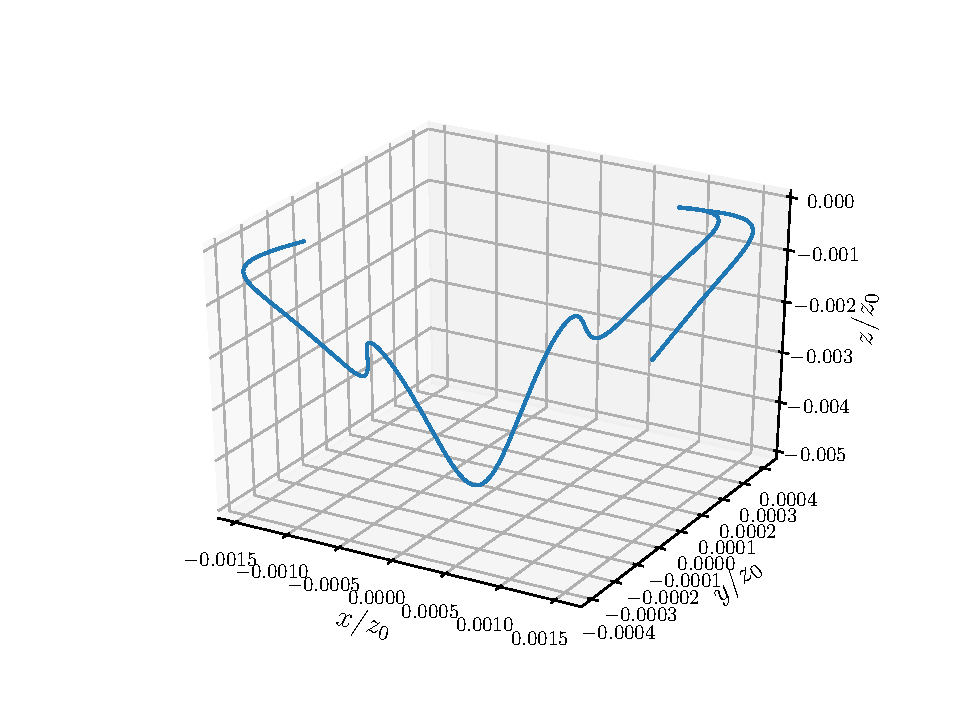
\includegraphics[width=0.8\linewidth]{figures/paul_trap_particles_only_one_total_time_0.1.pdf}}
  \caption{
  The 3D trajectory of a single particle in the Paul trap for $t = 0.1$ s. \label{fig:one_particle_trajectory}
  }
\end{figure}
%\clearpage % flush figures fig:one_particle_trajectory


% --- end solution of exercise ---

\subex{f)}
Suppose we place $N$ identical particles with charge $q > 0$ and mass $m$. Each particle, then, will experience a force from the field as well as from the electrostatic field formed by the charged particles themselves. Find the equations of motion for all the particles when you include the interaction between the particles and modify your code so it computes the position of all $N$ particles. Compute particle trajectories for $N = 2$, $N = 5$ and $N = 15$ particles and plot their trajectories in 3D. Are you able to trap multiple particles?


% --- begin solution of exercise ---
\paragraph{Solution.}
Let $\boldsymbol{F}_i$ denote the force on particle $i$. The force on the particle from the field setup by the trap is the same as before, that is:
\begin{equation}
  \boldsymbol{F}_{e,i} = \frac{2qV_0}{r_0^2}\cos(\Omega t)(x\hat{e}_x + y\hat{e}_y - 2z\hat{e}_z).
\end{equation}
The electric field created by all other particles except particle $i$ at particle $i$'s position is
\begin{equation}
  \boldsymbol{E}_i = \frac{1}{4\pi \epsilon_0}\sum_{j\neq i} q_j \frac{\boldsymbol{r}_i - \boldsymbol{r}_j}{|\boldsymbol{r}_i - \boldsymbol{r}_j|^3},
\end{equation}
where $\boldsymbol{r}_i$ denoted the position vector of particle $i$ and so on. The electric force due to this field on particle $i$ is just $\boldsymbol{F} = q\boldsymbol{E}$. The \emph{net} force on particle $i$ is thus
\begin{equation}
  \begin{split}
    \boldsymbol{F}_i & = \frac{2qV_0}{r_0^2}\cos(\Omega t)(x\hat{e}_x + y\hat{e}_y - 2z\hat{e}_z) + \frac{q_i}{4\pi \epsilon_0}\sum_{j\neq i} q_j \frac{\boldsymbol{r}_i - \boldsymbol{r}_j}{|\boldsymbol{r}_i - \boldsymbol{r}_j|^3} \\
    & = \frac{2qV_0}{r_0^2}\cos(\Omega t)(x\hat{e}_x + y\hat{e}_y - 2z\hat{e}_z) + \frac{q^2}{4\pi \epsilon_0}\sum_{j\neq i}  \frac{\boldsymbol{r}_i - \boldsymbol{r}_j}{|\boldsymbol{r}_i - \boldsymbol{r}_j|^3},
  \end{split}
\end{equation}
where I used that $q_i = q_j \equiv q$ and can thus be factorized out of the sum. Using Newton's 2.law $F = m\ddot{\boldsymbol{r}}$, then gives
\begin{equation}
  \ddot{\boldsymbol{r}} - \frac{2qV_0}{mr_0^2}\cos(\Omega t)(x\hat{e}_x + y\hat{e}_y - 2z\hat{e}_z) + \frac{q^2}{4\pi \epsilon_0 m}\sum_{j\neq i}  \frac{\boldsymbol{r}_i - \boldsymbol{r}_j}{|\boldsymbol{r}_i - \boldsymbol{r}_j|^3} = \boldsymbol{0},
\end{equation}
Modifying the class for the single-particle case we can create class with the following structure:
\begin{verbatim}
  class paul_trap:
      def __init__(self, Nparticles, total_time, Nsteps):
          self.Nparticles = Nparticles
          self.total_time = total_time
          self.Nsteps = Nsteps
          self.dt = total_time/Nsteps
          self.dt_squared = 0.5*self.dt**2
          elementary_charge = 1e-19
          self.g = 9.81           #m/s^2
          self.ke = 1./(4*np.pi*8.85e-12)         #Coulomb constant
          self.q_over_m = 1e-4             #C/kg
          self.m = 5e-5                  #Roughly the mass of a grain of cinnamon
          self.q = self.m*self.q_over_m    #Charge of a grain of cinnamon.
          self.v = np.zeros((Nparticles, Nsteps, 3)) #velocity
          self.r = np.zeros((Nparticles, Nsteps, 3)) #positions
          self.a = np.zeros((Nparticles,3))          #acceleration
          self.t = np.zeros(Nsteps)                  #time
          #Trap dimensions
          self.z0 = 0.005
          self.r0 = np.sqrt(2)*self.z0
          #AC source
          self.Omega = 2*np.pi*50         #50 Hz AC voltage.
          self.V0 = 4000                  #Volts
          for i in range(Nparticles):
              self.r[i, 0, :] = np.random.uniform(-0.5*self.z0, 0.5*self.z0, size=3)
      def solve_euler_cromer(self):
          bar = IncrementalBar("Progress", max = self.Nsteps)  #gives a neat progress bar
          for k in range(self.Nsteps-1):
              bar.next()
              self.t[k+1] = self.t[k] + self.dt
              omega_z = 4*self.q_over_m/self.r0**2*self.V0*np.cos(self.Omega*self.t[k])
              omega_xy = 0.5*omega_z
              for i in range(self.Nparticles):
                  self.a[i, 0] = omega_xy*self.r[i, k, 0]
                  self.a[i, 1] = omega_xy*self.r[i, k, 1]
                  self.a[i, 2] = -omega_z*self.r[i, k, 2] - self.g
                  #Add acceleration from interaction term:
                  F = np.zeros(3)
                  for j in range(self.Nparticles):
                      r_diff = np.zeros(3)
                      if i != j:
                          r_diff = self.r[i,k,:] - self.r[j,k,:]
                          rnorm = np.linalg.norm(r_diff)
                          F += r_diff/rnorm**1.5
                  F *= self.q*self.q_over_m*self.ke
                  self.a[i,:] += F
                  self.v[i, k+1, :] = self.v[i, k, :] + self.a[i, :]*self.dt
                  self.r[i, k+1, :] = self.r[i, k, :] + self.v[i, k+1, :]*self.dt
          bar.finish()
      def plot_trajectory(self):
          self.r[:,:,:]/self.z0
          fig = plt.figure()
          ax = fig.gca(projection='3d')
          ax.set_x\label(r"$x/z_0$", fontsize=14)
          ax.set_y\label(r"$y/z_0$", fontsize=14)
          ax.set_z\label(r"$z/z_0$", fontsize=14)
          for i in range(self.Nparticles):
              l = ["particle nr", str(i)]
              ax.plot(self.r[i,:,0], self.r[i,:,1], self.r[i,:,2], \label=" ".join(l))
          #plt.legend()
          l = ["paul_trap", "particles", str(self.Nparticles), \
                "total_time", str(self.total_time)]
          plt.savefig("_".join(l) + ".pdf")
          #plt.show()
          plt.close()
\end{verbatim}
which can be used in the following way (the file with the class is called particle\_system.py):
\begin{verbatim}
  from particle_system import paul_trap
  import sys
  Nparticles = 15
  total_time = float(sys.argv[1])
  Nsteps = int(1e5)
  my_trap = paul_trap(Nparticles, total_time, Nsteps)
  my_trap.solve_euler_cromer()
  my_trap.plot_trajectory()
\end{verbatim}
Figure~\ref{fig:2_particles} shows $N = 2$ particles for $t=0.1$ s. Figure~\ref{fig:5_particles} and figure~\ref{fig:15_particles} shows simulations carried over $t = 0.1$ s with $N = 5$ and $N = 15$ particles, respectively.


\begin{figure}[!ht]  % fig:2_particles
  \centerline{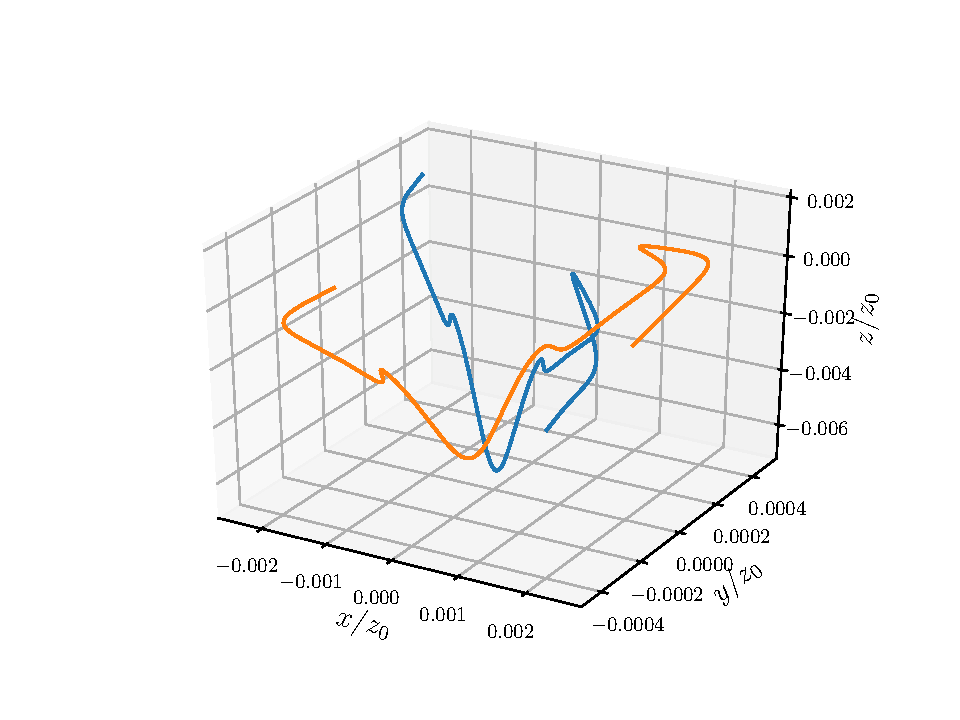
\includegraphics[width=0.8\linewidth]{figures/paul_trap_particles_2_total_time_0.1.pdf}}
  \caption{
  The 3D trajectory of a $N = 2$ particles for $t = 0.1$ s. \label{fig:2_particles}
  }
\end{figure}
%\clearpage % flush figures fig:2_particles



\begin{figure}[!ht]  % fig:5_particles
  \centerline{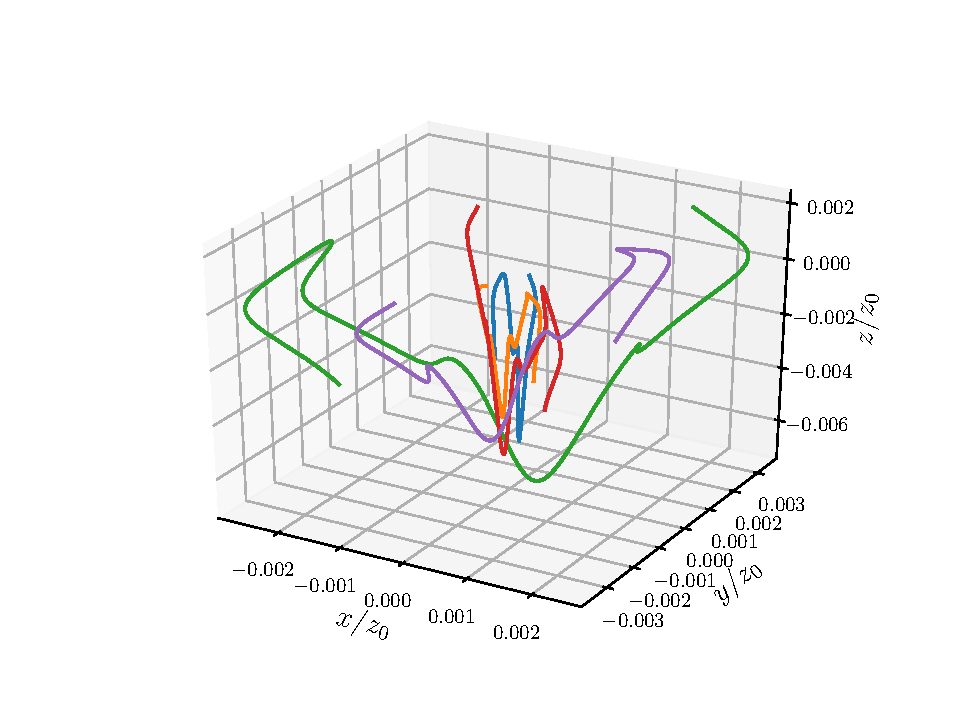
\includegraphics[width=0.8\linewidth]{figures/paul_trap_particles_5_total_time_0.1.pdf}}
  \caption{
  The 3D trajectory of a $N = 5$ particles for $t = 0.1$ s. \label{fig:5_particles}
  }
\end{figure}
%\clearpage % flush figures fig:5_particles



\begin{figure}[!ht]  % fig:15_particles
  \centerline{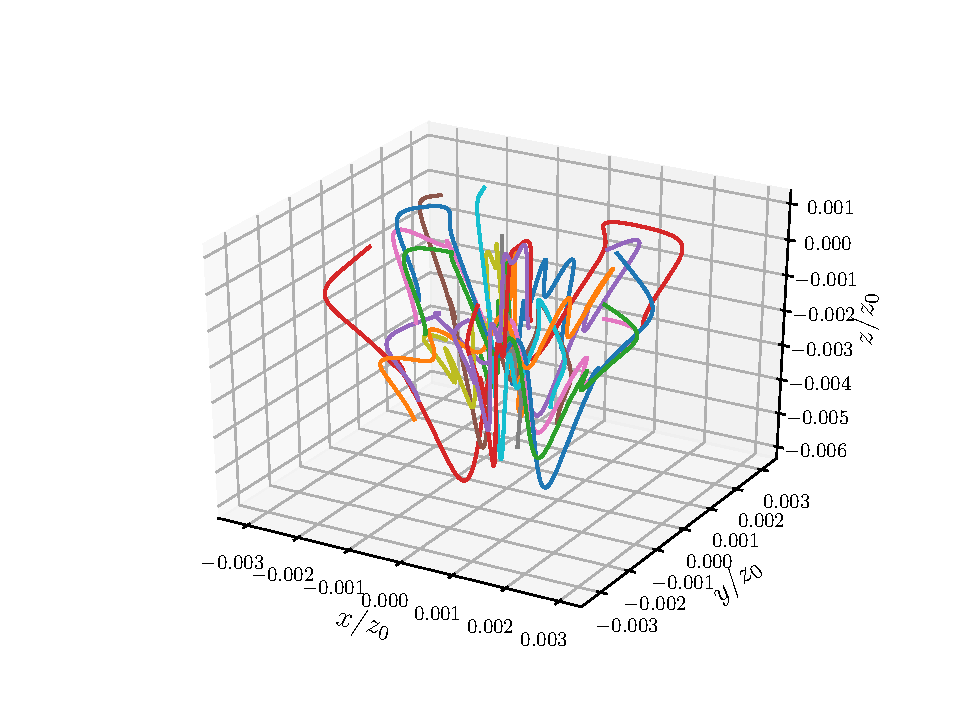
\includegraphics[width=0.8\linewidth]{figures/paul_trap_particles_15_total_time_0.1.pdf}}
  \caption{
  The 3D trajectory of a $N = 15$ particles for $t = 0.1$ s. \label{fig:15_particles}
  }
\end{figure}
%\clearpage % flush figures fig:15_particles


% --- end solution of exercise ---

\end{doconceexercise}
% --- end exercise ---


% ------------------- end of main content ---------------

% #ifdef PREAMBLE
\end{document}
% #endif

